% vim: set ft=tex

\chapter{\babDua}

Dalam bab ini, diuraikan dasar teori mengenai \tracking~serta sistem \pubsub.
Dasar teori tersebut digunakan untuk membangun sistem \tracking~multi target
yang efisien dengan arsitektur \pubsub.

\section{\f{Tracking}}

Pada umumnya proses \tracking~adalah proses mengamati orang atau benda yang
bergerak dan secara sekuensial mengirimkan data lokasi beserta
informasi-informasi lainnya.  Proses ini erat kaitannya dengan GPS (\GPS)
maupun sensor lokasi lainnya. Karena sifatnya yang sekuensial, dibutuhkan
proses \tracking~yang efisien namun tetap akurat.

\subsection{\f{Tracking} Pada Lingkungan Bergerak}

Proses \tracking~dikatakan ideal, apabila dapat mengirimkan perubahan lokasi
secara \f{robust} dalam kondisi yang berubah-ubah. Beberapa penelitian sebelumnya
(Civilis dkk, 2005) (Leonhardi dkk, 2001) (Leonhardi dkk, 2002) telah mengusulkan
adanya \tracking~secara dinamis untuk memperbarui lokasi. Dalam sistem EnTracked
(Kjaergaard dkk, 2010) sebuah sistem \tracking~yang efisien pada lingkungan
perangkat bergerak untuk target tunggal. Sistem ini dapat secara adaptif
menentukan kebutuhan presisi penentuan lokasi pada lingkungan bergerak. Penentuan
lokasi dapat memanfaatkan sensor GPS atau estimasi kecepatan obyek.

Target \tracking~dapat melibatkan satu obyek maupun lebih. Semakin banyak obyek
yang di-\tracking~maka semakin besar energi yang dibutuhkan dan pembaharuan
posisi yang terjadi. Perbedaan arah pergerakan, variasi kecepatan serta
konektifitas pada jaringan tak handal menjadi faktor utama dalam
\tracking~banyak obyek. (Ashfaque dkk, 2010) mengajukan metode
target kinematika dalam \tracking~pada lingkungan WSN (\wsn). Proses
\tracking~hanya aktif ketika sebuah obyek memasuki area tertentu.  Hanya pada
area \tracking, node sensor WSN yang aktif. Hal ini dapat mengurangi penggunaan
energi dan pengurangan \f{latency} pada jaringan.

\subsection{\f{Update Protocol}}

Terdapat beberapa metode \f{update protocol} yang dikenalkan dan mempunyai karakteristik
yang berbeda. Suatu protokol diasumsikan untuk memberbarui salinan informasi dari obyek
bergerak berdasarkan informasi obyek utama. Tujuannya adalah untuk menjamin akurasi informasi
yang diberikan. \f{Update protocol} dapat diklasifikasikan dalam tiga jenis, yaitu:
\f{querying}, \f{reporting} dan \f{combined}.

\noindent
\begin{figure}
  \centering
  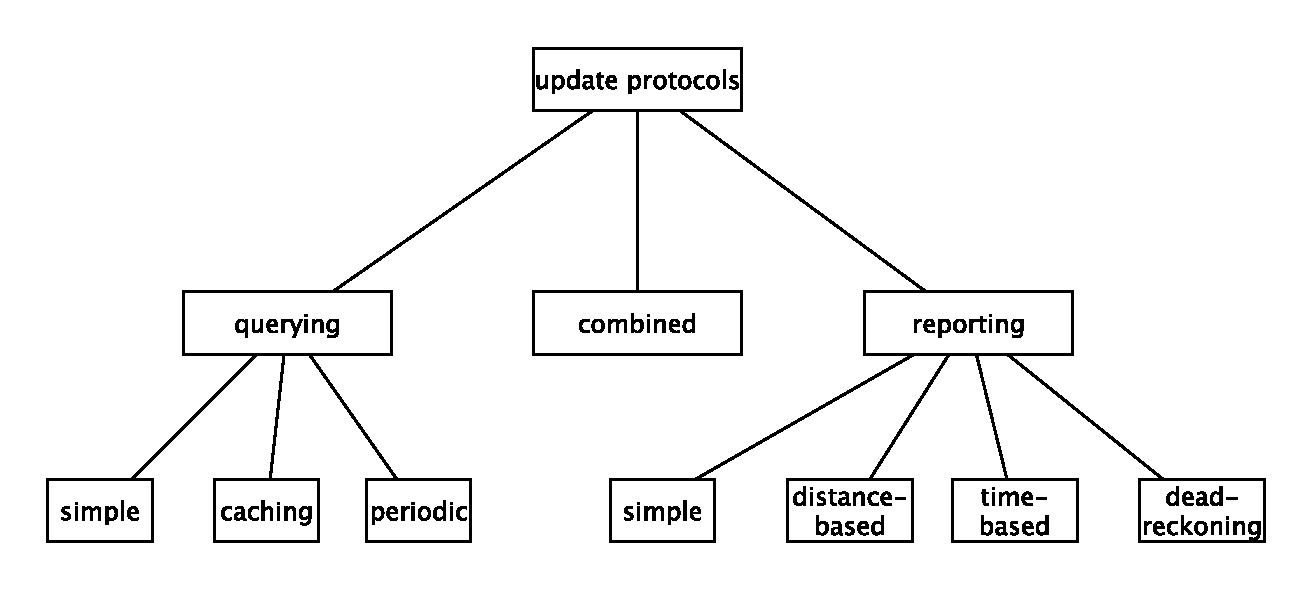
\includegraphics[scale=0.60]
  {images/2-klasifikasi}
\caption{Klasifikasi \f{Update Protocol} (Leonhardi dkk, 2001)}
\label{fig:sistem}
\end{figure}

% \noindent
% \begin{figure}
% \centering
%     \begin{tikzpicture}[font=\small, node distance=2cm, auto]
%         \node[draw] (update-protocols) {update protocols};
%         \node[draw, below of=update-protocols ] (combined) {combined};
%         \node[draw, left=2cm of combined] (querying) {querying};
%         \node[draw, right=2cm of combined] (reporting) {reporting};

        % \node[draw, below of=querying] (caching) {caching};
        % \node[draw, left=0.5cm of caching] (simple) {simple};
        % \node[draw, right=0.5cm of caching] (periodic) {periodic};

        % \node[draw, below of=reporting, align=center] (time-based) {time-\\based};
        % \node[draw, left=0.5cm of time-based, align=center] (distance-based) {distance-\\based};
        % \node[draw, left=0.5cm of distance-based] (simple-reporting) {simple};
        % \node[draw, right=0.5cm of time-based, align=center] (dead-reckoning) {dead-\\reckoning};

        % \path[line] (update-protocols) -- (querying);
        % \path[line] (update-protocols) -- (combined);
        % \path[line] (update-protocols) -- (reporting);

        % \path[line] (querying) -- (simple);
        % \path[line] (querying) -- (caching);
        % \path[line] (querying) -- (periodic);

        % \path[line] (reporting) -- (simple-reporting);
        % \path[line] (reporting) -- (distance-based);
        % \path[line] (reporting) -- (time-based);
        % \path[line] (reporting) -- (dead-reckoning);
    % \end{tikzpicture}
    % \caption{Klasifikasi \f{Update Protocol} (Leonhardi dkk, 2001)}
% \label{fig:update_protocols}
% \end{figure}

\begin{enumerate}
  [noitemsep
  ,nolistsep
  ,leftmargin=0cm
  ,itemindent=.5cm
  ,listparindent=\parindent
  ]
  \item \f{Querying Protocol}

        Sebuah protokol disebut \f{querying protocol} jika permintaan informasi lokasi
        dari sumber ditentukan oleh \f{server}. Sumber tidak perlu menyimpan informasi
        yang luas mengenai keadaan atau logika yang rumit. Jika informasi lokasi jarang
        diperlukan, protokol ini lebih efisien dibandingkan dengan protokol lain yang
        dipaparkan dalam Gambar~\ref{fig:update_protocols}. Terdapat tiga jenis protokol
        yang masuk dalam kategori ini yaitu: \f{simple}, \f{cached} dan \f{periodic}.

        \f{Simple}, \f{server} meminta informasi lokasi dari sumber setiap aplikasi memberikan
        \f{request}. Protokol ini memberikan akurasi informasi lokasi yang tinggi, tetapi
        juga memberikan jumlah pesan yang besar karena frekuensi dari \f{query}. Selain
        itu waktu respon \f{server} juga relatif besar, karena \f{server} harus menghubungi
        sumber untuk setiap \f{query}.

        \f{Cached}, protokol ini merupakan optimasi dari protokol \f{simple} dimana
        server menyimpan salinan informasi lokasi terakhir. \f{Server}
        melakukan estimasi apakah informasi terakhir masih cukup akurat, jika tidak
        \f{server} akan mengirimkan protokol \f{simple}.

        \f{Periodic}, jika sisi \f{server} mengirimkan \f{query} informasi lokasi
        secara periodik ke sumber dengan rentang waktu, protokol seperti ini
        disebut protokol \f{periodic}. Protokol ini memiliki kemiripan dengan jenis
        time-based pada protokol \f{reporting} yang akan dijelaskan selanjutnya.

    \item \f{Reporting Protocol}

        Perbedaan mendasar dengan \f{querying protocol} adalah pihak mana yang melakukan
        inisiasi. Pada \f{reporting protocol} pihak sumber akan memberikan pembaharuan
        jika telah mencapai suatu \f{threshold}. Pada umumnya \f{reporting protocol}
        memberikan akurasi yang lebih efisien dibandingkan protokol sebelumnya (lihat
        Tabel~\ref{tab:protokol}). Protokol ini dibagi menjadi tiga jenis,
        yaitu: \f{simple}, \f{time-based} dan \f{distance-based}.

        Pada protokol \f{simple}, pengiriman informasi lokasi terjadi setiap ada
        perubahan informasi, dikarenakan sebuah sensor mendapatkan informasi lokasi
        baru. Pada kasus ini, banyaknya pesan tergantung dari tingkat \f{update} dari
        sensor dan biasanya sangat tinggi.

        Sedangkan pada protokol \f{time-based}, informasi lokasi dikirimkan secara
        periodik setiap batas waktu T terlewati. Jumlah tingkat \f{update} bersifat
        tetap, tidak bergantung pada perilaku obyek bergerak. Jika obyek bergerak
        lambat, sedikit atau tidak ada perbedaan dalam informasi lokasi yang dikirimkan
        ke \f{server}. Dan jika obyek bergerak cepat, tidak cukup pesan yang dikirimkan
        untuk mencapai akurasi yang diinginkan.

\begin{table}
\centering\scriptsize
\caption{Perbedaan beberapa protokol (Leonhardi dkk, 2001)}
\label{tab:protokol}
\begin{tabular}{l >{\centering\arraybackslash}p{1.8cm}
                  >{\centering\arraybackslash}p{1.8cm}
                  >{\centering\arraybackslash}p{1.8cm}
                  >{\centering\arraybackslash}p{1.8cm}
                  >{\centering\arraybackslash}p{1.8cm}}
    \hline
    & Message rate depending on mobility& Message rate depending on queries&
    Upper bound for uncertainty of results& Applications may specify desired
    accuracy& Can detect disconnections \\
    \hline
    \bo{Querying:}  \\
    Simple           &   & x & (x) & x & x   \\
    Cached           &   & x & (x) & x & x   \\
    Periodic         &   &   &     &   & x   \\
    \\
    \bo{Reporting:} \\
    Simple           &   &   & (x) &   & (x) \\
    Time-based       &   &   &     &   & x   \\
    Distance-based   & x &   & x   &   &     \\
    Dead reckoning   & x &   & x   &   & x   \\
    \\
    \bo{Combined}    & x & x & x   & x & (x) \\
    \hline
\end{tabular}
\end{table}

        Protokol \f{distance-based} mengirimkan pembaharuan informasi lokasi
        ketika jarak antara lokasi dari obyek bergerak dan lokasi terakhir lebih
        besar dari \f{threshold} yang diberikan. Protokol ini akan memberikan
        lebih banyak pesan jika obyek bergerak cepat dan lebih sedikit jika
        bergerak pelan. Dimungkinkan juga untuk menggabungkan protokol
        \f{time-based} dan \f{distance-based}.

        Optimasi dari protokol \f{distance-based} adalah \f{dead-reckoning}.
        Server melakukan estimasi posisi sekarang dengan melihat posisi lama
        serta kecepatan dan arah pergerakan dari obyek. Sisi sumber juga
        melakukan estimasi lokasi dan mengirimkan pembaharuan jika informasi
        lokasi telah berbeda dari \f{threshold}.

    \item \f{Combined Protocol}

        \f{Querying protocol} tidak dapat menyesuaikan karakteristik pergerakan
        yang berbeda dari obyek bergerak, sedangkan \f{reporting protocol} tidak
        mempertimbangkan tingkat permintaan dan akurasi yang diminta oleh
        aplikasi. Dengan \f{combined protocol} yang mengintegrasikan
        \f{distance-based} dan \f{cached}, kedua kebutuhan di atas dapat
        terpenuhi. Jika informasi lokasi yang tersimpan pada \f{server} kurang
        akurat, server akan meminta informasi lokasi dari sumber.  Sedangkan
        sisi sumber mempunyai perilaku yang sama dengan \f{distance-based}.
        Dengan gabungan protokol ini, waktu respon bergantung pada seberapa
        akurat informasi yang tersimpan pada sisi server.

\end{enumerate}

\section{Location Model}
\label{sec:Location Model}

Dalam proses \tracking~diperlukan adanya yang disebut \locationmodel.
\LocationModel~adalah sebuah representasi yang ekspresif, fleksibel dan efisien
dari informasi lokasi (Leonhardi, 1998). Informasi lokasi tak lepas dengan
koordinat, yaitu penanda yang menentukan posisi sebuah obyek sehubungan dengan
referensi sistem koordinat yang diberikan (Becker, 2005). Sistem koordinat
terbagi menjadi dua, yaitu:

\begin{enumerate}[noitemsep, nolistsep]
    \item Koordinat geomatris yang mengacu pada titik geometris atau ruang multi dimensi
        seperti pada koordinat kartesius maupun koordinat geografis (\f{lattitude} dan
        \f{longitude}).
    \item Koordinat simbolis, mendefinisikan lokasi dalam bentuk simbol abstrak atau
        nama. Contoh: ``Jakarta'',``Surabaya'',``Ruang IF 105'' dan lain-lain.
\end{enumerate}

Dari kedua sistem koordinat diatas, \locationmodel~dibagi menjadi tiga macam, yaitu:
\f{Geometric}, \f{Symbolic} dan \f{Hybrid}.

\begin{enumerate}[noitemsep,nolistsep,leftmargin=0cm,itemindent=.5cm,listparindent=\parindent]
    \item \f{Geometric}

\f{Geometric location model} berbasiskan referensi koordinat sistem geometris.
Sebuah lokasi dapat direpresentasikan dalam suatu titik, area atau volume pada
sistem koordinat.  Relasi jarak dapat mudah didapatkan dengan penurunan
geometris menggunakan model matematika.

    \item \f{Symbolic}

\f{Symbolic location model} berbasiskan koordinat simbolis. Sebuah \f{symbolic
location} adalah nama yang bersifat simbol yang kehilangan referensi geometri.
Kumpulan dari beberapa koordinat dapat dikelompokkan dalam sebuah \f{symbolic
location}, misalnya: Gedung Jurusan Informatika. Beberapa pengembangan dari
\locationmodel~ini antara lain: \f{set-based}, \f{hierarchical},
\f{graph-based} dan \f{combined symbolic}.

    \item \f{Hybrid}

Perpaduan antara \f{symbolic location model} yang melampirkan koordinat dalam
sistem referensi. Terdapat dua pendekatan yaitu, \f{subspaces} dan \f{partial
subspaces}.  Perbedaan utama kedua pendekatan diatas adalah jumlah informasi
geometris yang disimpan.  \f{Partial subspaces} hanya menyimpan infomasi
geometris untuk beberapa lokasi saja.

\end{enumerate}

Setiap desain \locationmodel~mempunyai kelebihan dan kekurangan masing-masing,
hal ini dipaparkan pada Tabel~\ref{tab:locationmodel}. Tanda + menunjukkan
dukungan akan fungsi tersebut, semakin banyak tanda + menunjukkan kualitas yang
lebih baik.  Sedangkan tanda~-~bersifat sebaliknya. Adapun untuk kategori
\f{High}, \f{Medium}, dan \f{Very High} menunjukkan kompleksitas pemodelan
\locationmodel. Suatu desain \locationmodel~yang baik, desain yang dapat
memenuhi kebutuhan serta kompleksitas desain secara seimbang.

\begin{table}
  \centering\scriptsize
  \caption{Perbandingan \locationmodel~(Hinske, 2006)}
  \label{tab:locationmodel}
  \begin{tabular}
    {l >{\centering\arraybackslash}p{1.6cm}
      >{\centering\arraybackslash}p{0.6cm}
      >{\centering\arraybackslash}p{0.8cm}
      >{\centering\arraybackslash}p{1.8cm}
      >{\centering\arraybackslash}p{0.6cm}
      >{\centering\arraybackslash}p{0.6cm}
      >{\centering\arraybackslash}p{1cm}}
    \hline
    Location Model& Type& Position& Nearest neighbor& Navigation& Range&
    Modeling effort \\
    \hline
    Geometric                  & geo      & + & + & - & ++ & High \\
    Set-based                  & symb     & + & - & - & ++ & High \\
    Hierarchical               & symb     & + & - & - & ++ & Medium \\
    Graph-based                & symb     & + & + & - & ++ & Medium \\
    Combined symbolic          & symb     & + & + & - & ++ & High \\
    Subscpaces (Hybrid)        & symb/geo & ++ & ++ & - & ++ & Very high \\
    Partial subspaces (Hybrid) & symb/geo & ++ & +/++ & +/++ & +/++ & Very high \\
    \hline
  \end{tabular}
\end{table}
% \begin{figure}
%     \centering
%     \includegraphics[scale=0.5]
%         {pics/location-model-comparison.jpg}
%     \caption{Perbandingan \locationmodel~(Hinske, 2006)}
% \label{fig:location-model}
% \end{figure}

\section{\PubSub}

Skema interaksi \pubsub~mendapat perhatian yang cukup meningkat terutama dalam
interaksi skala besar. \Subscriber~dapat mendaftarkan ketertarikan suatu
\event~\pubsub~atau pola \event~\pubsub~yang dikirimkan oleh \publisher.
Kelebihan dari \f{event-based interaction} ini adanya sifat \decoupling~pada
waktu, ruang serta sinkronisasi antara \publisher~dan \subscriber.

Dasar dari model arsitektur pada interaksi
\pubsub~(Gambar~\ref{fig:arsitektur}) bergantung pada \f{event notification
service} yang menyediakan penyimpanan dan manajemen untuk \subscription~dan
pengiriman \event~\pubsub~secara efisien. \Subscriber~mendaftarkan ketertarikan
mereka yaitu \event~\pubsub~dengan memanggil operasi \subscribe() pada
\eventservice. Informasi \subscription~ini akan disimpan pada \f{event service}
tanpa disalurkan kepada \publisher. Operasi \unsubscribe() menghapus
\subscription~pada \eventservice. Untuk mengirimkan suatu \event~\pubsub,
\publisher~memanggil operasi \publish(). Setiap \subscriber~akan mendapat
notifikasi setiap \event~\pubsub~yang menjadi ketertarikannya.

\begin{figure}
    \centering
    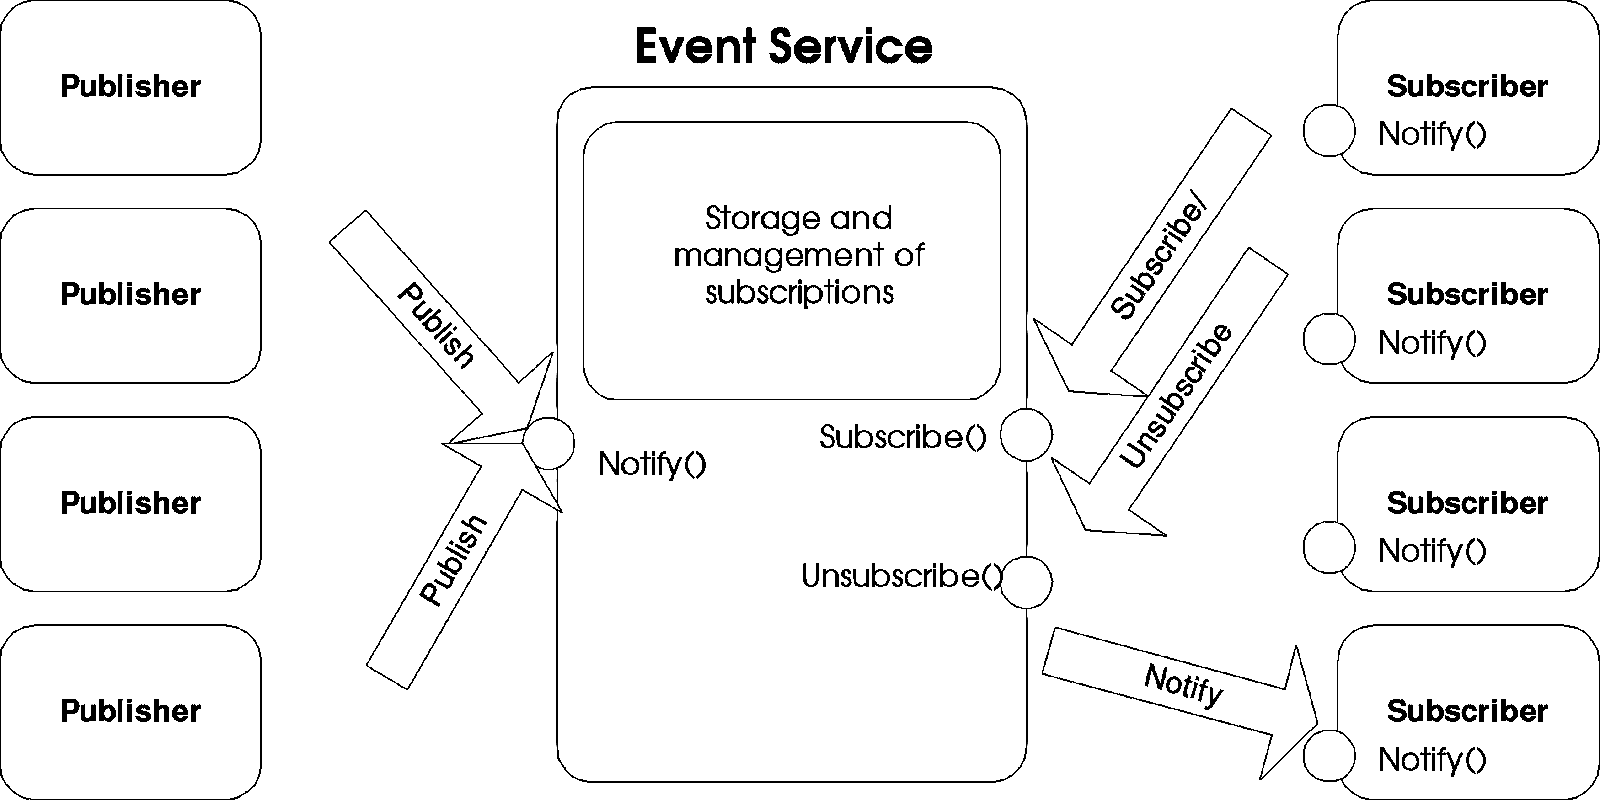
\includegraphics[scale=0.20]
    {images/2-arsitektur-pub-sub.png}
    \caption{Arsitektur dasar \pubsub~(Eugster dkk, 2003)}
\label{fig:arsitektur}
\end{figure}

\subsection{Dasar Skema Interaksi \PubSub}

Interaksi dalam sistem \pubsub~antara pihak \publisher~dengan \subscriber~yang
disediakan oleh \eventservice~terdapat \decoupling. Adanya \decoupling~ini
memberikan kelebihan pada sistem interaksi \pubsub~yang dapat didekomposisikan
menjadi tiga dimensi.  Untuk lebih jelasnya dapat dilihat pada
Gambar~\ref{fig:decoupling}.

\begin{enumerate}[noitemsep,nolistsep,leftmargin=0cm,itemindent=.5cm,listparindent=\parindent]
    \item \f{Space decoupling}

    Antara pihak yang berinteraksi tidak perlu saling mengetahui satu dengan
    yang lain. Para \publisher~mempublikasikan suatu \event~\pubsub~melalui
    \eventservice~dan para \subscriber~mendapatkannya secara tidak langsung
    melalui \eventservice.  Dalam interaksi ini antara \publisher~dan
    \subscriber~tidak saling mengetahui berapa jumlah yang terlibat.  \item \f{Time
    decoupling}

    Para pihak yang berinteraksi tidak perlu secara aktif berpartisipasi dalam
    interaksi pada waktu yang bersamaan. Pihak \publisher~mungkin
    mem-\publish~beberapa \event~saat \subscriber~terputus. Dan sebaliknya,
    \subscriber~mungkin akan mendapatkan notifikasi sementara \publisher~sedang
    terputus dari interaksi.  \item \f{Synchronization decoupling}

    Dalam interaksi antara pihak \publisher~dan \subscriber, \publisher~tidak diblok
    ketika mengirimkan suatu \event, dan \subscriber~mendapatkan pemberitahuan secara
    \asynch. Proses interaksi \event~tidak terjadi pada aliran kontrol utama antara
    \publisher~dan \subscriber~serta tidak terjadi secara sinkron.
\end{enumerate}
\begin{figure}
    \centering
    \includegraphics[scale=0.10]
        {images/decoupling.png}
    \caption{Jenis-jenis \f{decoupling} pada arsitektur \pubsub~(Eugster dkk, 2003)}
    \label{fig:decoupling}
\end{figure}

\subsection{Jenis-jenis \PubSub}
Umumnya \subscriber~hanya tertarik pada \event~\pubsub~tertentu, bukan semua \event~\pubsub.
Ada berbagai macam cara yang dapat digunakan dalam menentukan hal ini.
Dua skema yang paling banyak digunakan yaitu, \topicbased~serta \contentbased.

\begin{enumerate}[noitemsep,nolistsep,leftmargin=0cm,itemindent=.5cm,listparindent=\parindent]
    \item \TopicBased

        Merupakan jenis skema \pubsub~pertama
        yang berdasarkan topik atau subyek. Ketertarikan \subscriber~diidentifikasi
        dengan kata kunci. Pengembangan dari skema jenis ini dengan adanya hirarkis
        topik. Ketertarikan pada suatu topik termasuk sub-topik yang berada di bawahnya.
        Selain itu ketertarikan pada suatu topik dapat juga berupa \f{wildcard}, hal ini
        pertama kali diperkenalkan pada TIBCO \f{Rendezvous}. Nama topik pada umumnya
        dinotasikan dalam bentuk seperti URL, misalnya: \f{Eurecom/Courses/DSMWare}.
        Kelemahan skema ini bersifat statis, kriteria topik sudah didefinisikan.
    \item \ContentBased

        Skema \subscription~pada jenis ini, ketertarikan didasarkan pada isi dari
        suatu \event~\pubsub.
        Pada umumnya propertinya berisi atribut dari data struktur. Skema jenis ini
        lebih dinamis dari \topicbased. Dalam skema ini terdapat
        suatu bahasa dalam menentukan \subscription, contohnya: ``\f{Course=DSMWare and
        Grade\textless10}''.
    \item Type-Based Publish/Subscribe

        Suatu topik biasanya dikelompokkan tidak hanya berdasarkan kemiripan yang muncul,
        tetapi juga dalam suatu struktur. Hal ini yang mendasari adanya klasifikasi
        yang menyaring suatu \event~\pubsub~berdasarkan jenisnya.
\end{enumerate}

%\subsection{\PubSub~pada Lingkungan Perangkat Bergerak}

%Kebanyakan penelitian dalam sistem \pubsub~sejauh ini berfokus pada jaringan
%tak bergerak. Gucola dkk (Gucola dkk, 2000) berpendapat bahwa kelebihan sistem
%\pubsub~dapat diterapkan dalam lingkungan perangkat bergerak maupun nirkabel.
%Sifat dinamis pada sistem \pubsub~memungkinkan sistem untuk cepat beradaptasi
%dengan kondisi koneksi yang tidak stabil pada \f{mobile node}, yang merupakan
%karakteristik dari jaringan selular. Sifat asinkronitas sangat membantu, karena
%perangkat bergerak yang sering dimatikan atau terputus dari jaringan untuk
%jangka waktu yang lama. Ditambah lagi karateristik perangkat nirkabel yang
%memiliki kemampuan serta \f{bandwidth} yang terbatas. Sifat \f{multicasting}
%sistem \pubsub~membantu dalam sistem skala besar.

%Dengan meningkatnya popularitas perangkat bergerak, perlu adanya adaptasi dalam
%sistem \pubsub~pada lingkungan perangkat bergerak (Huang dkk, 2001)
%(Gambar~\ref{fig:content-based}). Sebagai contoh penerapannya, pada medan
%perang militer, ribuan sensor nirkabel dan mobile melaporkan segala macam
%informasi mulai dari lokasi pasukan musuh serta kondisi peralatan perang.
%Seorang tentara mungkin perlu mengetahui lokasi pasukan musuh terdekat atau
%timnya.  Hal-hal di atas memerlukan penyebaran komunikasi berskalabitas tinggi
%dalam infrastruktur dinamis yang sangat cocok dengan sistem \pubsub.

%\begin{figure}
    %\centering
    %\includegraphics[scale=0.40]
        %{pics/event-brokering-system.png}
    %\caption{Sistem \f{content-based publish/subscribe (Huang dkk, 2001)}}
    %\label{fig:content-based}
%\end{figure}

%\begin{figure}
    %\centering
    %\includegraphics[scale=0.40]
        %{pics/centralized-architecture.png}
    %\caption{Arsitektur terpusat, pencocokan serta penyaringan dilakukan sebuah server}
    %\label{fig:central}
%\end{figure}

\subsection{Protokol MQTT}

Protokol MQTT (MQ \f{Telemetry Transport}) adalah sebuah protokol \pubsub~yang
didesain sangat sederhana dan ringan. Protokol ini desain untuk perangkat
dengan \f{resource} terbatas, \f{low-bandwidth}, \f{high-latency} atau jaringan
yang tak handal. Protokol ini ditemukan oleh Dr Andy Stanford-Clark dari IBM
dan Arlen Nipper dari Arcom pada tahun 1999. Hunkeler dkk (Hunkeler dkk, 2008)
melakukan adaptasi protokol MQTT pada lingkungan WSN (\f{Wireless Sensor
Network}). Lingkungan WSN membutuhkan suatu protokol yang ramah energi serta
\f{low-bandwidth}. Beberapa kelebihan protokol ini dalam lingkungan WSN,
komunikasi data berdasarkan ketertarikan bukan dari suatu alamat perangkat
serta dapat menyembunyikan topologi jaringan. Protokol ini memungkinkan adanya
komunikasi antara WSN dan jaringan terdahulu maupun antar WSN yang berbeda.
Karakteristik lingkungan WSN dapat disejajarkan dengan lingkungan bergerak,
sehingga dalam penelitian ini akan digunakan protokol MQTT.

% ActiveMQ (sebuah \f{messaging queue framework}) yang dirilis oleh Apache
% menyediakan kemudahan dalam membangun sistem \pubsub. ActiveMQ mendukung
% bermacam client bahasa pemrograman dan protokol. Selain dukungan di atas,
% \framework~ini telah teruji pada server J2EE yang umum dikenal. ActiveMQ
% dibangun menggunakan bahasa Java, sehingga mewarisi kelebihan dari bahasa
% pemrograman Java. Dan selain itu, protokol MQTT sudah didukung oleh
% \framework~ini.

\section{\Context~\Aware}

Untuk membangun sistem yang adaptif diperlukan adanya \context~\aware.
\Context~didefinisikan sebagai informasi yang dapat digunakan untuk
menggambarkan situasi dari entitas (Hong dkk, 2009). Entitas disini dapat
berupa orang, tempat atau obyek yang dianggap relevan untuk interaksi antara
pengguna dengan aplikasi termasuk lokasi, waktu, aktivitas dan preferensi.
Sebuah sistem dapat dikategorikan dalam \context~\aware~jika sistem dapat
mengekstrak serta menterjemahkan menggunakan informasi dari \context~sert
aterdapat fungsi yang dapat beradaptasi pada \context~yang digunakan. Dalam
pengertian yang lebih sederhana, sebuah sistem disebut \context~\aware~jika
sistem menggunakan \context~untuk memberikan informasi yang relevan kepada
pengguna, dimana relevansi tergantung pada kegiatan pengguna.

\subsection{\Acc}

Sensor \acc~adalah sebuah alat yang berfungsi untuk mengukur percepatan dan
getaran akibat gravitasi bumi. Percepatan merupakan suatu keadaan berubahnya
kecepatan terhadap waktu dimana terjadi perubahan kecepatan yang semakin
bertambah daripada kecepatan sebelumnya.  Hal ini disebut dengan
\f{acceleration}. Percepatan juga bergantung pada arah/orientasi karena
merupakan penurunan kecepatan yang merupakan besaran vektor. Berubahnya arah
pergerakan suatu benda akan menimbulkan percepatan pula. Pembagian sumbu pada
\acc~dibagi menjadi sumbu \f{x}, \f{y} dan \f{z} (\f{triaxial accelerometer}).
Aktifitas pengguna yang berbeda menghasilkan nilai yang berbeda pula,
dipengaruhi interaksi antara pengguna dan sensor.

Dengan memanfaatkan sensor \acc~dapat dideteksi aktifitas seorang pengguna.
Randell dkk (Randell dkk, 2000) mengumpulkan data sampel sumbu \f{x} dan \f{y}
pada \acc. Data sampel dari 10 orang, berisi tentang aktifitas pengguna dalam
berbagai aktifitas: berjalan, berlari, duduk, berjalan naik tangga, turun
tangga dan berdiri. Dari data yang dikumpulkan, dianalisa untuk mengetahui pola
aktifitas menggunakan algoritme \f{clustering}.

\subsection{\f{Activity Recognition}}

\f{Activity recognition} merupakan teknik yang digunakan dalam proses
klasifikasi aktifitas fisik pengguna (berjalan, duduk atau berlari). Dalam
proses ini terbagi menjadi beberapa tahapan, yaitu: \f{data collection},
\f{feature extraction} dan \f{data interpretation}. Untuk melakukan sebuah
klasifikasi diperlukan adanya data.  Data yang diperoleh disesuaikan dengan
\context~yang digunakan. Pada umumnya pengambilan data dilakukan dengan
menggunakan sebuah alat yang berupa sensor. Dari data yang didapatkan melalui
sensor, proses selanjutnya adalah ekstraksi data. Data yang akan diklasifikasi
diolah sedemikian rupa sehingga data tidak terlalu konvergen atau divergen.
Kemudian tahapan terakhir yaitu klasifikasi, tahapan yang terpenting dalam
pengenalan aktifitas pengguna.

Mengacu pada konsep \tracking~yang ideal, maka diperlukan mekanisme penentuan
lokasi yang ramah energi. Suatu mekanisme yang dapat secara adaptif menentukan
tingkat kebutuhan presisi suatu lokasi. Dalam kondisi bergerak, diperlukan
ketelitian posisi yang lebih baik. Pergerakan dapat dideteksi memanfaatkan
sensor \acc~yang telah diajukan oleh You dkk (You dkk, 2008). Mekanisme ini
kemudian diadopsi pada sistem EnTracked (Kjaergaard dkk, 2009). Sistem
EnTracked hanya mendeteksi dua kondisi pergerakan, yaitu: diam berdiri atau
bergerak. Ketika terjadi pergerakan yang terdeteksi, perubahan lokasi
ditentukan menggunakan sensor GPS. Diagram alir untuk deteksi pergerakan
\f{tracking} dipaparkan pada Gambar~\ref{fig:movement}.

\begin{figure}
    \centering
    \begin{tikzpicture}[font=\small, node distance=2cm, auto]
        \node[cloud] (start) {Start};
        \node[block, below of=start] (gpspos) {Get GPS Position};
        \node[block, below of=gpspos] (report) {Report Position to Server};
        \node[decision, below of=report] (device) {Is device moving?};
        \node[block, right=3cm of start] (speedgps) {Determine Speed with GPS};
        \node[block, below of=speedgps] (timelimit) {Determine Time Limit};
        \node[block, below of=timelimit] (consumption) {Minimize Consumption};
        \node[block, below of=consumption] (schedule) {Schedule Features};
        \node[decision, below of=schedule] (schedulegps) {Schedule GPS now?};

        \coordinate(A) at ($ (gpspos) + (-3, 0) $);
        \coordinate(B) at ($ (report) + (-2.5, -1.5) $);
        \coordinate(C) at ($ (start) + (2.5, 0) $);
        \coordinate(D) at ($ (schedule) + (3, -1.5) $);

        \path[line] (start) -- (gpspos);
        \path[line] (gpspos) -- (report);
        \path[line] (report) -- (device);

        \path[line] (device.west) -| (B) -- node [near start] {False} ($(report) + (0,-1.5)$);
        \path[line] (device.east) -| (C) -- node [near start] {True} (speedgps.west);
        \path[line] (speedgps) -- (timelimit);
        \path[line] (timelimit) -- (consumption);
        \path[line] (consumption) -- (schedule);
        \path[line] (schedule) -- (schedulegps);

        \path[line] (schedulegps) -| (A) -- node [near start] {True} (gpspos);
        \path[line] (schedulegps) -| (D) -- node [near start] {False} ($(schedule) +(0,-1.5)$);
    \end{tikzpicture}
    \caption{Diagram alir untuk mendeteksi pergerakan (Kjaergaard dkk, 2010)}
    \label{fig:movement}
\end{figure}

\section{Location API Sistem Operasi Android}

Saat ini, \smartphone~seperti Android sudah dilengkapi dengan GPS untuk
menentukan lokasi. Dalam menentukan lokasi, tidak hanya memanfaatkan GPS saja,
tetapi dapat juga dengan memanfaatkan Cell-Id atau WiFi. Sistem operasi Android
sudah menyediakan \f{Location API}, sebuah API (\api) yang dapat membantu dalam
menentukan lokasi. API ini terdapat dalam \f{package} \f{android.location}.
Terdapat dua kelas utama yang berperan dalam penentuan lokasi yaitu \locM~dan
\locP. \Class~\locM~menyediakan akses layanan lokasi pada Android.  Layanan ini
memungkinkan untuk mengakses penyedia lokasi. Sedangkan \class~\locP~menentukan
metode apa yang digunakan untuk memperoleh lokasi. Beberapa metode yang
tersedia dijabarkan pada Tabel~\ref{tab:provider}.

\begin{table}
\centering
\caption{Jenis-jenis \locP}
\label{tab:provider}
\begin{tabular}{l p{9cm}}
        \hline
        \locP~& Deskripsi \\
        \hline
        network & \Provider~ini menentukan lokasi berdasarkan ketersedian menara seluler
        dan akses WiFi. Mungkin memiliki presisi lebih tinggi dibandingan dengan GPS
        dalam ruang tertutup.\\
        gps & \Provider~ini menentukan lokasi menggunakan satelit. Tergantung pada kondisi,
        \provider~ini mungkin memerlukan waktu untuk mendapatkan lokasi yang tepat.
        Pada umumnya memliki presisi lebih baik dibandingan dengan \network.\\
        passive & \Provider~ini dapat digunakan secara pasif dalam menerima perubahan
        lokasi di saat aplikasi atau layanan lain meminta perubahan posisi. \Provider~ini
        mengembalikan lokasi yang dihasilkan oleh \provider~lain.\\
        \hline
    \end{tabular}
\end{table}

Selain metode-metode \provider~di atas, penentuan lokasi dapat dilakukan secara
fleksibel dengan menggunakan \provider~terbaik menggunakan \f{Criteria}. Dalam
penentuan lokasi \provider~membutuhkan akses dari sistem pada android, yang
diatur dalam ACCESS\_COARSE\_LOCATION serta ACCESS\_FINE\_LOCATION
(\provider~gps). Ketika akses ACCESS\_FINE\_LOCATION digunakan, akses
ACCESS\_COARSE\_LOCATION tidak diperlukan.
